%%%%%%%%%%%%%%%%%%%%%%%%%%%%%%%%%%%%%%%%%%%%%%%%%%%%%%%%%%%%%%%%%%%%%%
% How to use writeLaTeX: 
%
% You edit the source code here on the left, and the preview on the
% right shows you the result within a few seconds.
%
% Bookmark this page and share the URL with your co-authors. They can
% edit at the same time!
%
% You can upload figures, bibliographies, custom classes and
% styles using the files menu.
%
%%%%%%%%%%%%%%%%%%%%%%%%%%%%%%%%%%%%%%%%%%%%%%%%%%%%%%%%%%%%%%%%%%%%%%

\documentclass[12pt]{article}

\usepackage{sbc-template}

\usepackage{graphicx,url}

%\usepackage[brazil]{babel}   
\usepackage[utf8]{inputenc} 

\usepackage{float}
\usepackage{hyperref}
     
\sloppy

\title{VsCode + Platform.io + Semáforo}

\author{Fabricio Araújo Dias}

\address{Instituto Federal de Educação, Ciência e Tecnologia do Ceará
  (IFCE)\\
  Avenida Vice-Presidente José Alencar, S/N -- 61.939-140 -- Maracanaú -- CE -- Brasil
  \email{fabricio.araujo61@aluno.ifce.edu.br}
}

\begin{document} 

\maketitle

\begin{abstract}
  This report describes step-by-step the first practical activity of the Microcontrollers course, which consists of setting up the development environment on the machine, writing a code in C++ that will make an LED turn on and off constantly and sending it to the ESP32 microcontroller. Full operation will also be reported.
\end{abstract}
     
\begin{resumo} 
  Esse relatório descreve o passo a passo da primeira atividade prática da disciplina de Microcontroladores que consiste em definir o ambiente de desenvolvimento na máquina, escrever um código em C++ que fará um LED ligar e desligar constantemente e enviar para o microcontrolador ESP32. Assim como o pleno funcionamento também será relatado.
\end{resumo}


\section{Configurando Ambiente de Desenvolvimento}

A máquina utilizada possui componentes desprezíveis para a realização da prática. Seu sistema operacional é Linux e utiliza a distribuição Lubuntu - com a adição de nenhum outro programa que não venha pré-instalado. 

Foi escolhido o editor de texto Visual Studio Code (VSCode) como editor de código. Ele não veio pré-instalado com o Lubuntu, então foi necessário realizar o download do instalador na página oficial e a instalação foi feita utilizando o gerenciador de pacotes APT pelo terminal.

Com o VSCode instalado, ele será usado junto com a extensão PlatformIO IDE extension. A PlatformIO é uma ferramenta criada para o desenvolvimento de projetos para sistemas embarcados que auxilia a escrita do código e facilita o envio para o microcontrolador. A extensão realiza a instalação da ferramenta na máquina, cria uma integração da ferramenta com o VSCode e faz com que ele funcione como uma IDE.

O PlatformIO necessita do Python instalado junto com o módulo venv para a criação de ambientes virtuais, e ele foi instalado pelo terminal com instruções da paǵina oficial do PlatformIO.

Feito isso, a configuração do ambiente de desenvolvimento está concluída.

\section{Criação do Projeto e Desenvolvimento do Código}

\begin{figure}[H]
    \centering
    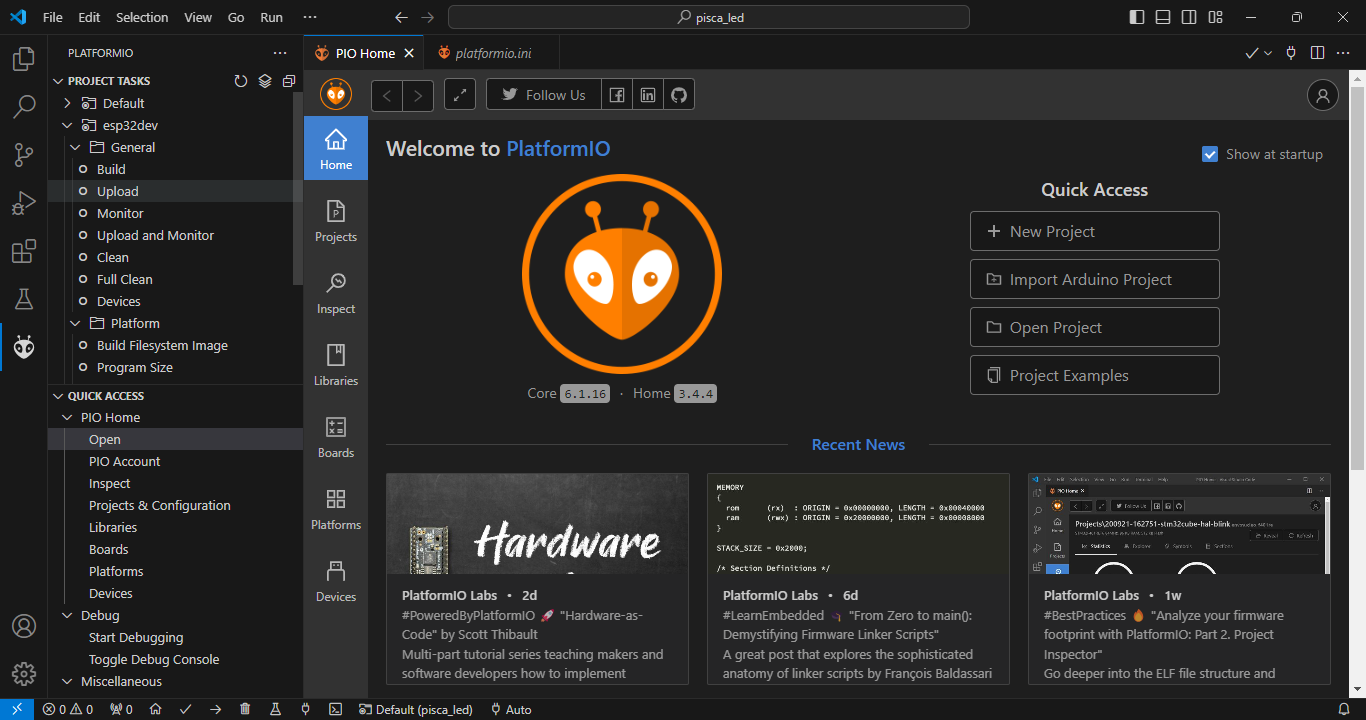
\includegraphics[width=0.5\linewidth]{img/Captura de tela 2024-10-27 171928.png}
    \caption{Tela inicial do PlatformIO no VSCode.}
    \label{fig:platformIO-home}
\end{figure}

\begin{figure}[H]
    \centering
    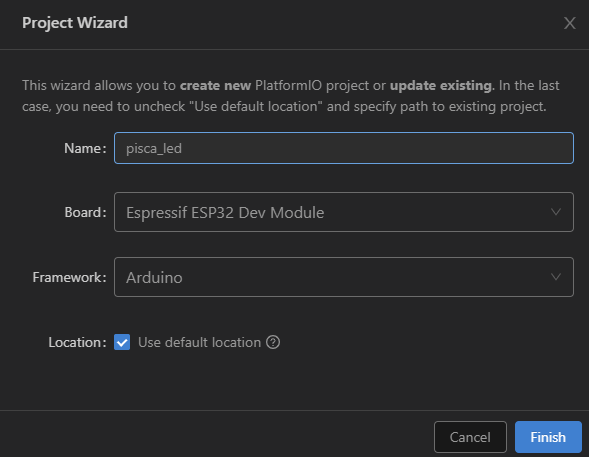
\includegraphics[width=0.5\linewidth]{img/Captura de tela 2024-10-27 172116.png}
    \caption{Wizard para criar um novo projeto no PlatformIO.}
    \label{fig:platformIO-wizard}
\end{figure}

O primeiro projeto fará simplemente um LED acender e desligar dado um período de tempo. Utilizando a extensão do PlatformIO no VSCode, entramos na página inicial da ferramenta e criamos o projeto. Na tela de escolhas, definimos o título do projeto como pisca\_led, a placa como Espressif ESP32 Dev Module e o framework como Arduino. O projeto passou a ser criado e receber suas configurações básicos. Teve uma demora considerável.

Ao terminar, a extensão irá mudar automaticamente o ambiente de trabalho para a pasta do projeto. Na pasta src, há o arquivo main.cpp onde será implementado o código de execução. No arquivo, há duas funções sem retorno: uma função se chama setup onde será feito a configuração dos pinos do microcontrolador; e a outra função se chama loop que funciona como um laço while.

Em setup, escolhemos o pino 18 para conectar ao LED e configuramos esse mesmo pino para saída utilizando a função pinMode com os parâmetros 18 e OUTPUT.

Em loop, desenvolvemos o código simples para fazer o LED acender, esperar, apagar, esperar, acender, etc. Utilizamos a função digitalWrite para acionar ou cessar a tensão no pino correspondente do LED - HIGH para acionar e LOW para cessar. Para que o LED acenda e apague com um atraso, colocamos uma função delay com 1000 no parâmetro depois de cada digitalWrite para esperar por 1 segundo antes de ir para a próxima linha de execução.

Para conferir o código, acesse o \href{https://github.com/fabricio-araujo94/microcontroladores/blob/main/pisca_led/}{código no Github}.

Assim, o código está pronto e só é necessário enviar para o ESP32. Pode ser feito pela paleta de comandos ou utilizando o atalho ALT + SHIFT + U. Antes disso, é necessário preparar o microcontrolador.

\section{Preparação do Microcontrolador ESP32 e Resultado}

Além do ESP32 de 30 pinos com entrada serial micro-USB e um cabo micro-USB, foram utilizado uma protoboard de 400 pontos, um resistor, um LED comum e dois cabos macho-fêmea.

\begin{figure}[H]
    \centering
    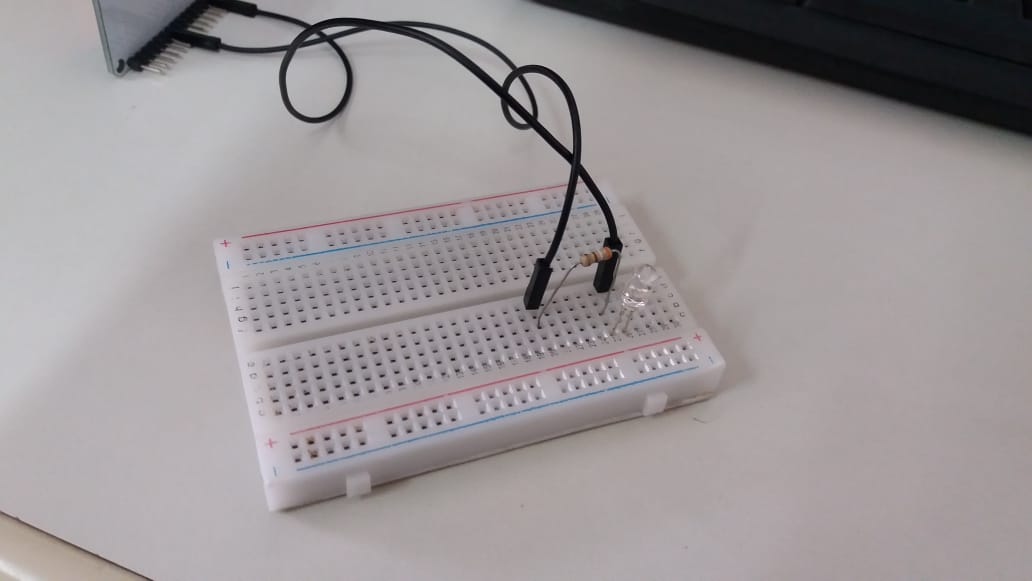
\includegraphics[width=0.5\linewidth]{img/Imagem do WhatsApp de 2024-10-25 à(s) 22.05.44_680386d1.jpg}
    \caption{Configuração na protoboard}
    \label{fig:protoboard}
\end{figure}

\begin{figure}[H]
    \centering
    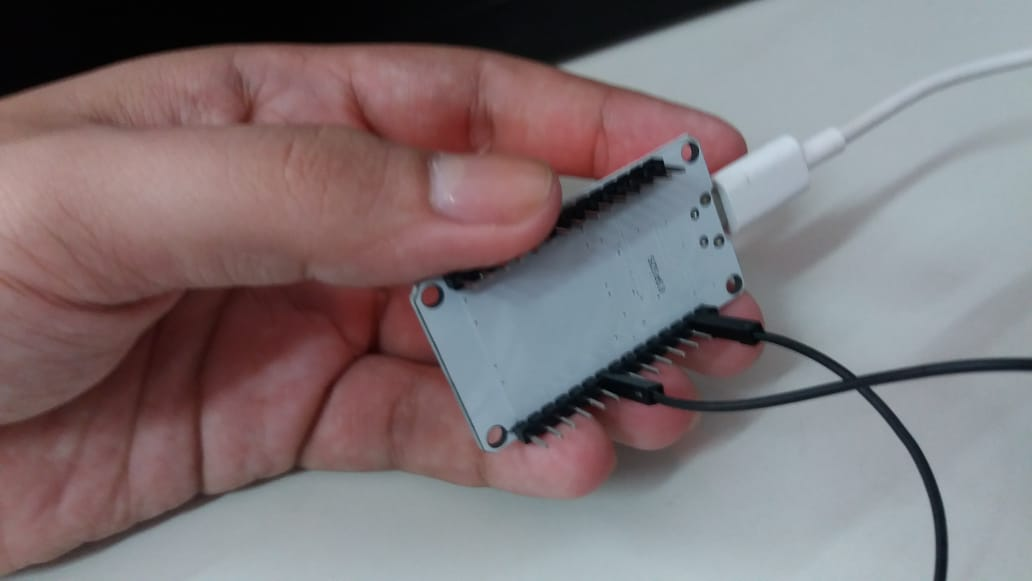
\includegraphics[width=0.5\linewidth]{img/Imagem do WhatsApp de 2024-10-25 à(s) 22.05.44_a72b281d.jpg}
    \caption{Configuração nos pinos do ESP32.}
    \label{fig:esp32-pins}
\end{figure}

Como foi dito na seção do código em C++, o pino de ESP32 escolhido arbitrariamente foi o pino 18. Então, conectamos o lado fêmea do cabo no pino 18 e o lado macho do cabo em um ponto qualquer da protoboard. Na coluna onde foi conectado o cabo, adicionamos um terminal do resistor para que não ocorra risco de queimar o LED e o outro terminal em um próximo numa coluna diferente. Então, na coluna onde ficou o outro terminal do resistor, adicionamos o terminal positivo do LED e o outro terminal também fica num ponto próximo em outra coluna. Por fim, pegamos o outro cabo e conectamos o macho em um ponto da coluna onde foi ligado o terminal negativo do LED e conectados a parte fêmea no pino GND.

Realizando todo esse processo, o LED deverá acender e apagar num invervalo de 1 segundo.

Para conferir o resultado final em vídeo, assista o \href{https://youtu.be/n_IYHKFdlQg}{vídeo no Youtube}.

\begin{figure}[H]
    \centering
    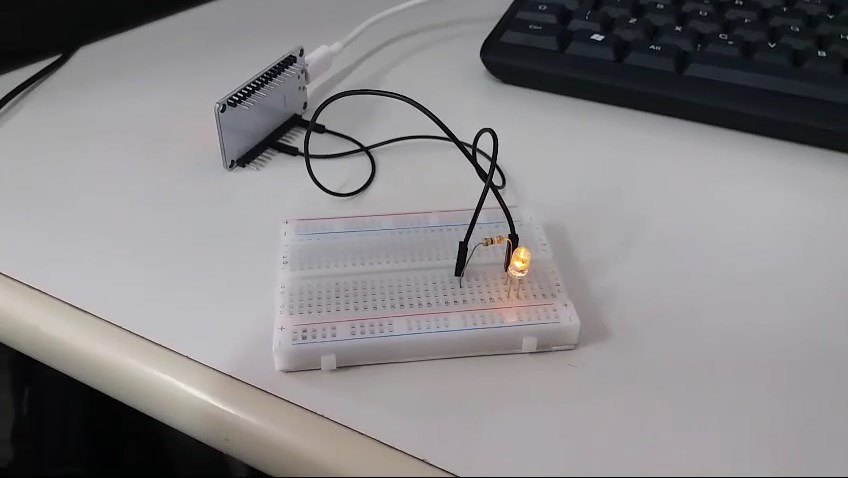
\includegraphics[width=0.5\linewidth]{img/Vídeo do WhatsApp de 2024-10-25 à(s) 22.05.43_c4fb24fe.mp4_snapshot_00.02.438.jpg}
    \caption{Resultado final.}
    \label{fig:result}
\end{figure}



\end{document}
